\documentclass[aspectratio=169]{beamer}
\usepackage[english]{babel}
\usepackage[utf8]{inputenc}
\usepackage{verbatim}
\usepackage{graphicx}
\usepackage{pgfpages}
\usepackage{ulem}
\usepackage{float}
\usepackage{amsmath}

\setbeameroption{hide notes}

\setbeamercolor{title}{fg=white}
\setbeamercolor{author}{fg=white}
\setbeamercolor{normal text}{fg=black}
\setbeamercolor{frametitle}{fg=black}
\setbeamercolor{item}{fg=red}
\setbeamercolor{block title}{fg=red}
\setbeamercolor{section in toc}{fg=red}
\setbeamercolor{footline}{fg=white}
\setbeamercolor{title in head/foot}{fg=white,bg=black}

\setbeamertemplate{navigation symbols}{}
\setbeamertemplate{headline}{
    
\includegraphics[height=1mm, width=\paperwidth]{wg-headline.png}
}

\setbeamertemplate{footline}{
    \begin{beamercolorbox}[ht=1.2em]{title in head/foot}
        {\footnotesize \hspace{1em}\inserttitle, \insertshortauthor}
    \end{beamercolorbox}
}

\begin{document}

\title{World of Tanks: Linux and Open Source Inside}
\author{Maksim Melnikau}
\date{}

{
\title{
    
\includegraphics[width=0.4\textwidth]{wg-logo.png}
    \\
    {\huge World of Tanks\\Linux and Open Source Inside}
}
\usebackgroundtemplate{
\includegraphics[width=\paperwidth]{wg-end.jpg}}
\begin{frame}[plain]{}
    \titlepage
\end{frame}
}

\usebackgroundtemplate{
\includegraphics[width=\paperwidth]{wg-bg.jpg}}
\logo{
    
\includegraphics[height=1.7cm]{wg-logo.png}
}

\section{Intro}
\begin{frame}{I'm}
    \begin{itemize}
        \item developer in Wargaming (Belarus, Minsk)
            \begin{itemize}
                \item \sout{Order of War}
                \item \sout{Order of War: Challenge}
                \item World of Tanks
            \end{itemize}

        \item Linux Mobile hobbyist
            \begin{itemize}
                \item \sout{Openmoko}
                \item systemd
                \item telepathy
                \item Gentoo
            \end{itemize}
    \end{itemize}
\end{frame}

\begin{frame}{World of Tanks}
    \begin{itemize}
        \item mmorpg
        \item fps about tanks
        \item 15x15 pvp 
    \end{itemize}
\end{frame}

\begin{frame}{World of Tanks Today}
    \begin{itemize}
        \item 800k concurrent users in peak
        \item 8M messages per second
        \item 500 servers for game and web
        \item 60M game portal visits per month
        \item 5 PB (petabytes) for game installs and updates per month
    \end{itemize}
\end{frame}

\section{Big Project --- Big Problems}
{
\usebackgroundtemplate{
\includegraphics[height=\paperheight]{pain.jpg}}
\begin{frame}[plain]{}
\end{frame}
}

\begin{frame}{Cheaters}
    \begin{itemize}
        \item many players want to cheat
        \item cheaters make other players unhappy
        \item cheaters xenophobia
    \end{itemize}
\end{frame}

\begin{frame}{Scaleability}
    \begin{itemize}
        \item better product --- more users
        \item more users --- more servers
        \item more servers --- bigger synchronization problem
    \end{itemize}
\end{frame}

\begin{frame}{Single Datacenter Issues}
    \begin{itemize}
        \item latency
        \item availability
        \item single point of failure
    \end{itemize}
\end{frame}

\begin{frame}{Big Data}
    \begin{itemize}
        \item more users --- more data
        \item more data --- bigger disks
        \item suddenly, new storage solution required
    \end{itemize}
\end{frame}

\begin{frame}{Rapid Growth}
    \begin{itemize}
        \item simple solution --- faster time to market
        \item great success --- simple solutions completely unusable
        \item rewriting everything on-the-fly
        \item business changes every day
    \end{itemize}
\end{frame}

\section{Ideas}
{
\usebackgroundtemplate{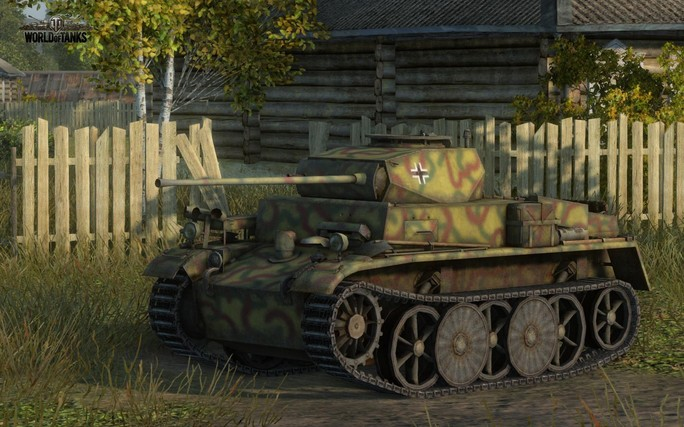
\includegraphics[width=\paperwidth]{ideas.jpg}}
\begin{frame}[plain]{}
\end{frame}
}
\begin{frame}{Nobody Will Help You}
    \begin{itemize}
        \item no time to educate people
        \item no time to wait 3rd party support
        \item no time to write good proper solutions
    \end{itemize}
\end{frame}

\begin{frame}{Full Control}
    \begin{itemize}
        \item software
        \item data
        \item team
        \item hardware
    \end{itemize}
\end{frame}

\begin{frame}{Linux and Open Source Software}
    \begin{itemize}
        \item ready to use components 
        \item good documentation
        \item customize software when required
        \item hire people with required skills
    \end{itemize}
\end{frame}

\section{World of Tanks Internals}
{
\usebackgroundtemplate{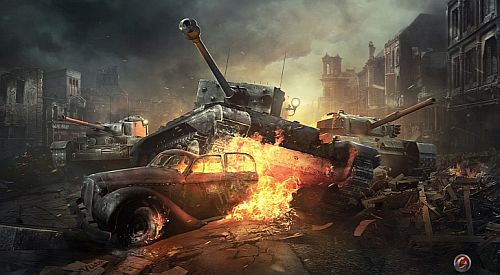
\includegraphics[height=\paperheight]{dev.jpg}}
\begin{frame}[plain]{}
\end{frame}
}
\begin{frame}{World of Tanks Architecture}
    \begin{itemize}
        \item game client --- thin client, player
        \item server --- world simulation
        \item cluster --- thousands of process working as one server
        \item step-game world, with very small steps
    \end{itemize}
\end{frame}

\begin{frame}{Development}
    \begin{itemize}
        \item regular Python
        \item GC disabled
        \item some parts rewritten on C++
        \item message-based RPC
        \item UDP-based reliable internal protocol
    \end{itemize}
\end{frame}

{
\logo{}
\begin{frame}{Cluster}
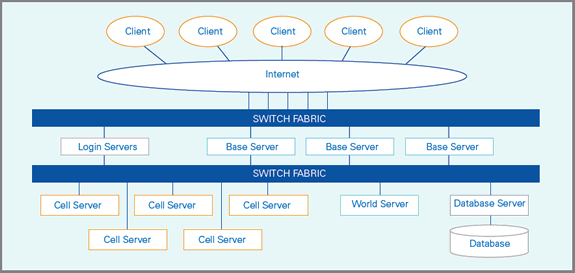
\includegraphics[width=\textwidth]{server.png}
\end{frame}
}

\begin{frame}{Multi Cluster}
    \begin{itemize}
        \item scaleability
        \item geo distributed
        \item availability
        \item independence
    \end{itemize}
\end{frame}

\begin{frame}{Production}
    \begin{enumerate}
        \item 500 servers
        \item 8k cpu cores
        \item 32 TB RAM 
        \item Linux
    \end{enumerate}
\end{frame}

\begin{frame}{MySQL}
    \begin{itemize}
        \item database size: 300 GB
        \item 384 GB RAM
        \item Percona 5.5 (buffer pool warming --- 1GBps)
        \item 40k selects, 1k inserts, 1k updates per second
        \item 24 HDD $*$ 600 GB $*$ 0.5 = 6 TB
    \end{itemize}
\end{frame}

\begin{frame}{Client}
    \begin{enumerate}
        \item regular Python
        \item HUD - ActionScript, Scaleform
        \item 3D graphics - C++
    \end{enumerate}
\end{frame}


\section{Forgotten}
{
\usebackgroundtemplate{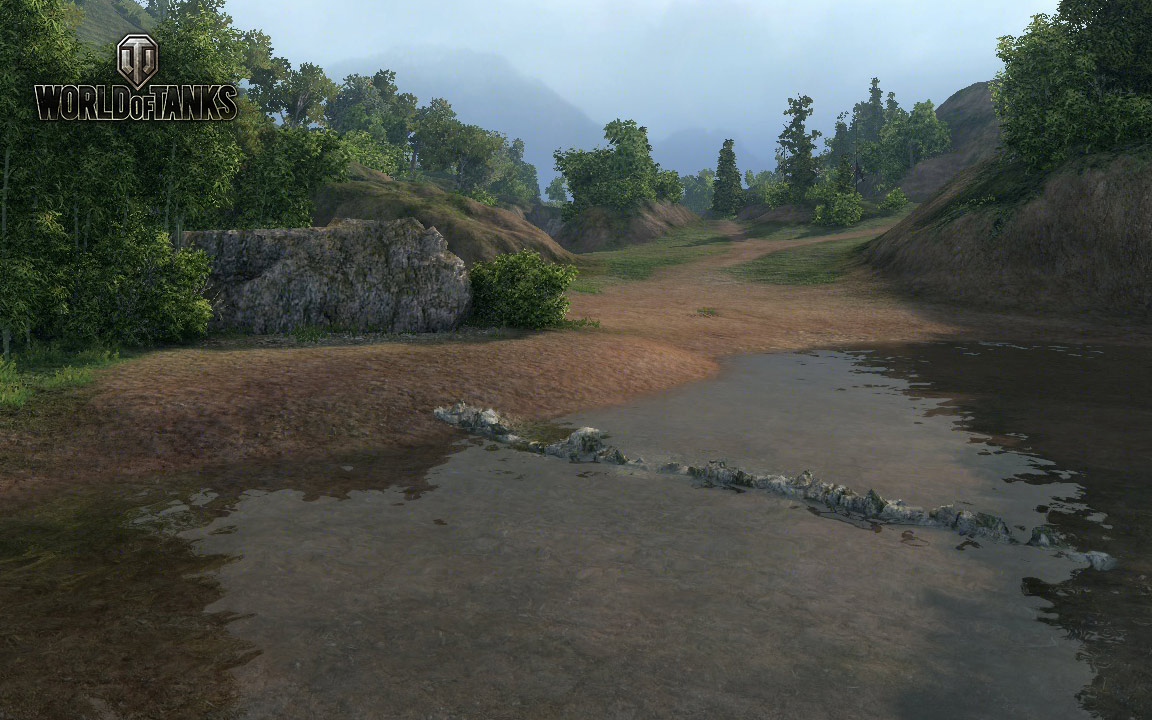
\includegraphics[width=\paperwidth]{forgotten.jpg}}
\begin{frame}[plain]{}
\end{frame}
}

\begin{frame}{Web Tasks}
    \begin{columns}
        \begin{column}{0.4\textwidth}
        \begin{itemize}
            \item registrations
            \item news
            \item docs
            \item media
            \item payment form
            \item receiving payments
        \end{itemize}
        \end{column}
    
        \begin{column}{0.4\textwidth}
        \begin{itemize}
            \item update distribution
            \item account management
            \item account profile
            \item statistics
            \item ratings
            \item ...
        \end{itemize}
        \end{column}
    \end{columns}
\end{frame}

\begin{frame}{LNAMPMR}

\includegraphics[width=0.2\textwidth]{linux-logo.png}\hspace{0.5cm}

\includegraphics[width=0.2\textwidth]{nginx-logo.png}\hspace{0.5cm}

\includegraphics[width=0.2\textwidth]{apache-logo.png}\hspace{0.5cm}

\includegraphics[width=0.2\textwidth]{mysql-logo.png}
\vspace{0.5cm}

\includegraphics[width=0.2\textwidth]{python-logo.png}\hspace{0.5cm}

\includegraphics[width=0.2\textwidth]{memcached-logo.png}\hspace{0.5cm}

\includegraphics[width=0.2\textwidth]{rabbitmq-logo.png}\hspace{0.5cm}
\end{frame}

\begin{frame}{Other}

\includegraphics[width=0.2\textwidth]{uwsgi-logo.png}\hspace{0.5cm}

\includegraphics[width=0.2\textwidth]{twisted-logo.png}\hspace{0.5cm}

\includegraphics[width=0.2\textwidth]{php-logo.png}\hspace{0.5cm}

\includegraphics[width=0.2\textwidth]{ruby-logo.png}
\vspace{0.5cm}

\includegraphics[width=0.2\textwidth]{postgresql-logo.png}\hspace{0.5cm}

\includegraphics[width=0.2\textwidth]{mongodb-logo.png}\hspace{0.5cm}

\includegraphics[width=0.2\textwidth]{redis-logo.png}\hspace{0.5cm}
\end{frame}

{
\usebackgroundtemplate{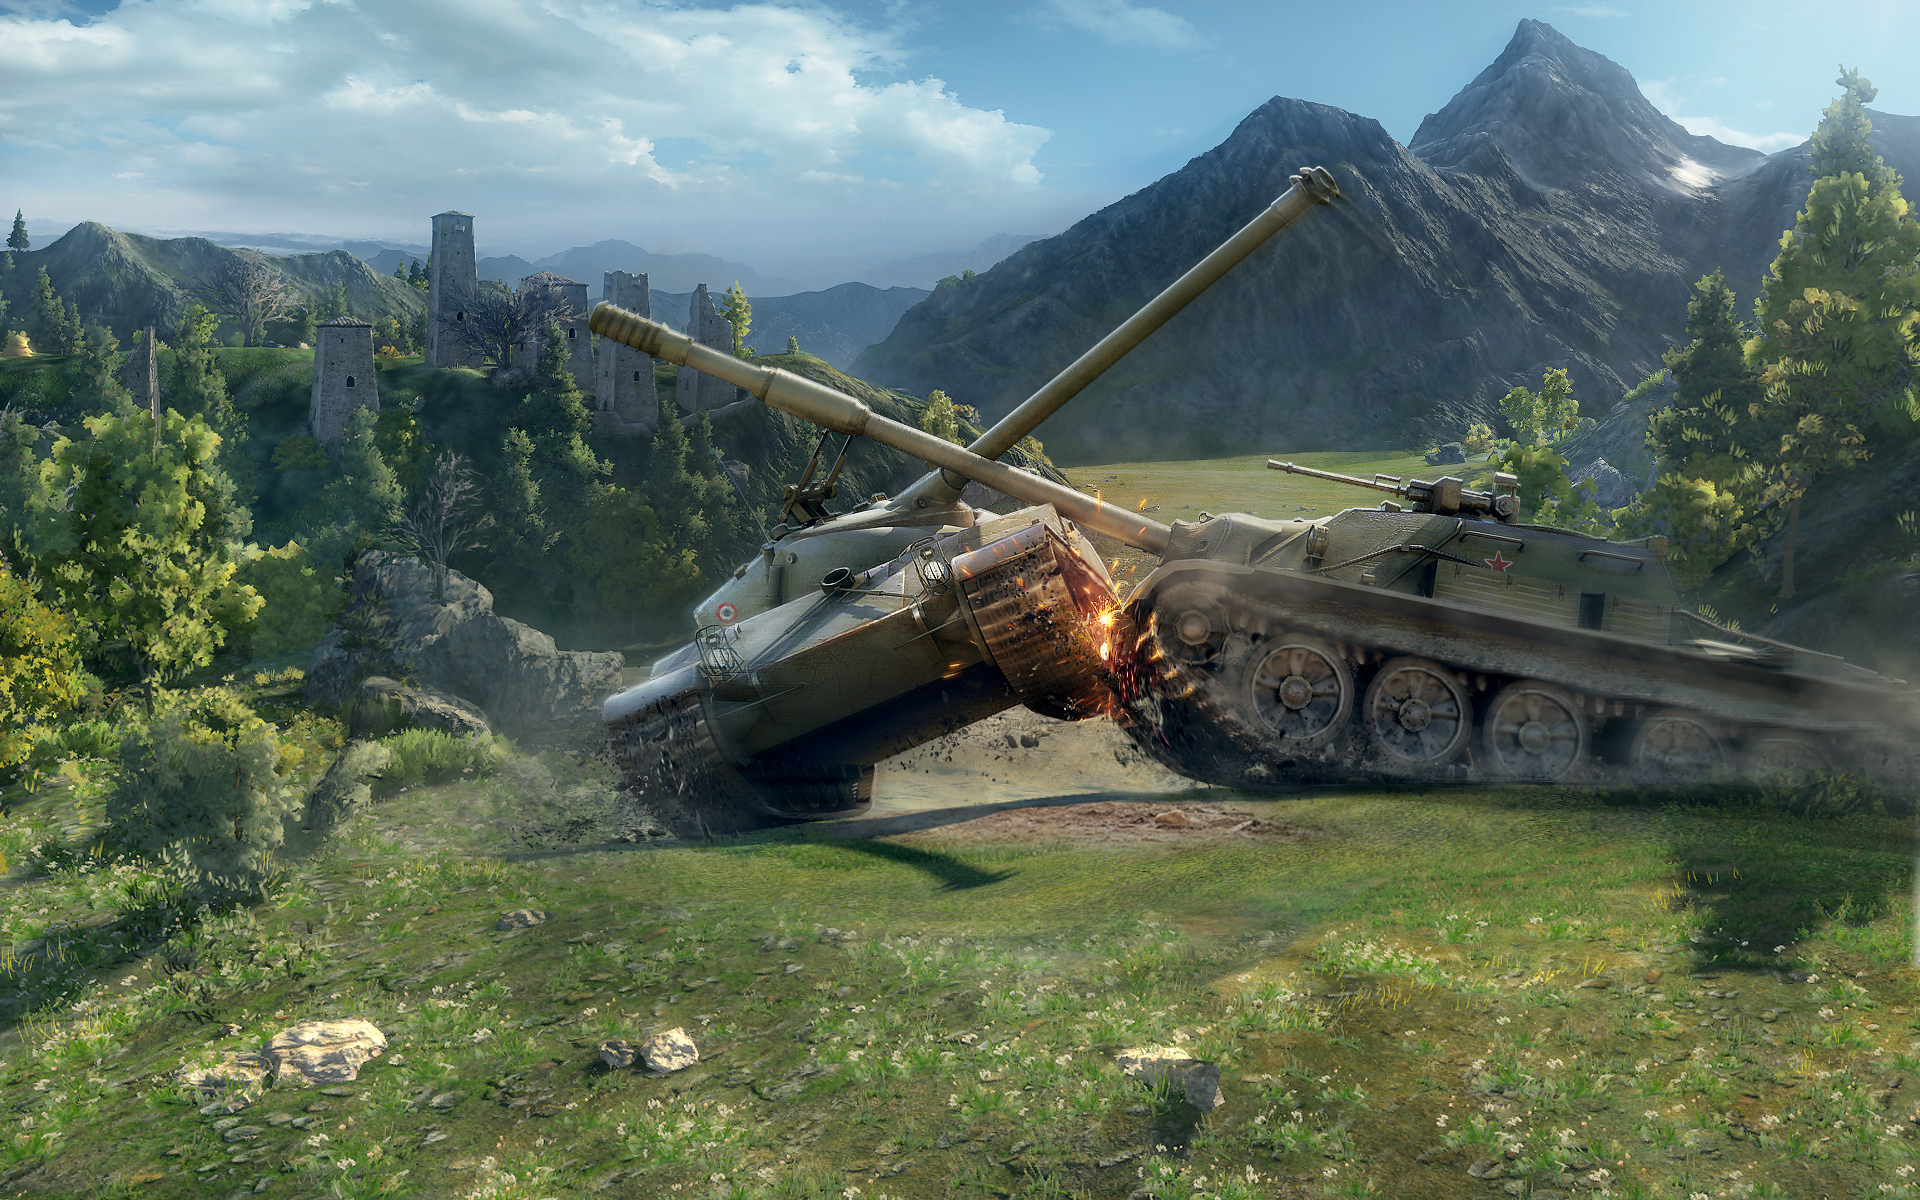
\includegraphics[width=\paperwidth]{wot.jpg}}
\begin{frame}[plain]{}
\end{frame}
}

\begin{frame}{Keys to Success}
    \begin{itemize}
        \item Linux on server
        \item relaying on Open Source
        \item fast and easy development
        \item having full control on everything
        \item don't afraid of different software stacks
    \end{itemize}
\end{frame}

{
\setbeamertemplate{footline}{}
\setbeamercolor{frametitle}{fg=white}
\setbeamercolor{normal text}{fg=white}
\setbeamercolor{block title}{fg=white}
\setbeamercolor{block body}{fg=red}

\usebackgroundtemplate{
\includegraphics[height=\paperheight]{wg-end.jpg}}
\begin{frame}{Thank You. Questions}
    \begin{block}{Maksim Melnikau}
    \par \url{mailto:m\_melnikau@wargaming.net}
    \par \url{https://plus.google.com/114669104565190507739/}
    \par \url{https://twitter.com/max\_posedon}
    \par \url{http://wargaming.com}
    \end{block}
\end{frame}
}

\end{document}
